\documentclass[12pt,a4paper]{article}

\usepackage{float}
\restylefloat{figure}
\usepackage{hyperref}
\usepackage{graphicx}
\usepackage{gensymb}
\usepackage[title]{appendix}
\usepackage[dotinlabels]{titletoc}
\usepackage[nottoc,numbib]{tocbibind}
\usepackage{mathtools}
\usepackage[margin=0.5in]{geometry}
\renewcommand{\thefootnote}{\arabic{footnote}}

\newcommand*\wrapletters[1]{\wr@pletters#1\@nil}
\def\wr@pletters#1#2\@nil{#1\allowbreak\if&#2&\else\wr@pletters#2\@nil\fi}

\usepackage{enumitem}
\setenumerate{itemsep=0pt}

% Add support for multi-page tables.
\usepackage{longtable}

\pagenumbering{arabic}

\title{EE4DSA Coursework 4}
\author{Chris Cummins}

\begin{document}
\maketitle

\section{Implementing the Fibonacci Program}

In order to write the Fibonacci program for the $\mu C$ architecture,
the rather unimaginatively named UCASM assembler was written. The
assembler performs the translation from human readable assembly code
into machine code, with a syntax and instruction set inspired by AVR
Assembler. See \texttt{extra/ucasm-ref.pdf} for full usage
instructions and details. The source code for the assembler command
line and web interfaces are included in \texttt{extra/ucasm}.

The file \texttt{extra/ram.asm} contains the source code for my
implementation of the Fibonacci sequence program. The program
generates the next number in the Fibonacci sequence every time the
user presses the centre button, and the output number is displayed on
the four digit seven segment display. If the number exceeds 4 decimal
digits in length, then the seven segment display will scroll through
the digits from left to right. LEDs 2-8 are used to indicate which 4
digits digits are currently being displayed, and LED 1 is lit to
indicate a series reset or overflow. For example, the decimal number
$1234567$ would be displayed by scrolling through the four most
significant digits as such:

\begin{table}[H]
  \centering
  \begin{tabular}{ c c }
    \textbf{LED} & \textbf{SSD} \\
    00000\textbf{1}000 & 1234 \\
    000000\textbf{1}00 & 2345 \\
    0000000\textbf{1}0 & 3456 \\
    00000000\textbf{1} & 4567 \\
    00000\textbf{1}000 & 1234 \\
    000000\textbf{1}00 & 2345 \\
  \end{tabular}
\end{table}

\subsection{Computing the Fibonacci sequence}

A number in the Fibonacci sequence can be calculated using nearest
integer rounding:

$$F(n) = \left[\frac{\phi^n}{\sqrt{5}}\right] $$

Where $n$ is the index of the number in the series. We can use this to
approximate the number of bits required to store the Fibonacci number
$F(n)$ in binary encoding by rearranging for $\log(F(n))$:

$$\log(F(n)) \approx n \times \log(\phi) - \log(\sqrt{5})$$

Where $\log(\phi) \approx 0.694$ and $\log(\sqrt{5}) \approx
0.35$. For large $n$ values, the significance of $\log(\sqrt{5})$
tends towards $0$, allowing us to calculate the number of bits
required as:

$$\log(F(n)) = \lceil 0.694n \rceil$$

For the $\mu C$ architecture we can substitute $\log(F(N))$ with the
32-bit word size and solve for $n$ to determine the largest index in
the Fibonacci sequence that we can store in a single word:

$$n = \lceil \frac{32}{0.694} \rceil = 47$$

This means that in order to avoid integer overflow, our iterative
Fibonacci algorithm must enforce a strict upper bound:

$$F(n) = F(n - 1) + F(n - 2), 0 \le n \le 47$$

When $n = 47$, the sequence resets.

\subsection{Optimisation details}

The software was written with ``correct style'' as the primary goal,
not performance. Specific decisions that were made at the expense of
clock cycles include:

\begin{itemize}
\item Each interrupt handler preserves the state of the registers it
  uses, despite the register file being easily large enough to
  allocate dedicated registers to each ISR. Removing the stack
  activity from the ISRs would reduce the execution time
  significantly, since each register push/pop pair adds an extra 6
  clock cycles to the execution time.
\item Data which is shared between both ISRs and the main program
  logic is stored in RAM. This is not required since the register file
  is large enough to store all program data. Placing all data in
  registers would allow for immediate access without the need for the
  load / store instructions.
\item The lack of caching means that there is no benefit to exploiting
  temporal locality in memory accesses, so instructions are ordered to
  make the best chronological sense, not to reduce data hazards. The
  lack of instruction caching also means that there is never any
  benefit to using fixed length loops instead of unrolling them.
\item Interrupt handlers and subroutines are written to operate on as
  small of a register footprint as possible, due to the slow push/pop
  operations.
\end{itemize}

Beyond this, the main performance caveat is the binary to binary coded
decimal conversion, which is performed by repeatedly dividing the
binary number $n$ by decreasing powers of ten for every BCD digit, as
shown in the following pseudo-code:

\begin{verbatim}
def bin2bcd(n):
        i = NO_OF_BCD_DIGITS - 1
        while i > 0:
                d      = i ^ 10
                bcd[i] = n / d
                n      = n % d
                i     -= 1
        bcd[0] = n
\end{verbatim}

The limited support for hardware integer arithmetic means that the
division has to be performed in software using iterative subtraction:

\begin{verbatim}
def div(n, divisor):
        i = 0

        while n > divisor:
                n -= divisor
                i += 1

        ret i
\end{verbatim}

This means that the BCD conversion operates in $O(n^2)$ time
complexity, where $n$ is the number of output BCD digits - 1. While
this clearly does not scale well for very large input numbers, this is
acceptable for our purposes, where the small and constant value of $n
= 9$ means that the worst case input requires only 81 subtractions.

\section{Software testing}

A test bench was written (see \texttt{extra/test\_bench.vhd}) which
runs a complete simulation of all program bevahiour \footnote{I
  wouldn't recommend running the testbench as it takes well over 10
  minutes to complete even on a 4.5GHz monster!}, demonstrating:

\begin{figure}[H]
  \centering
  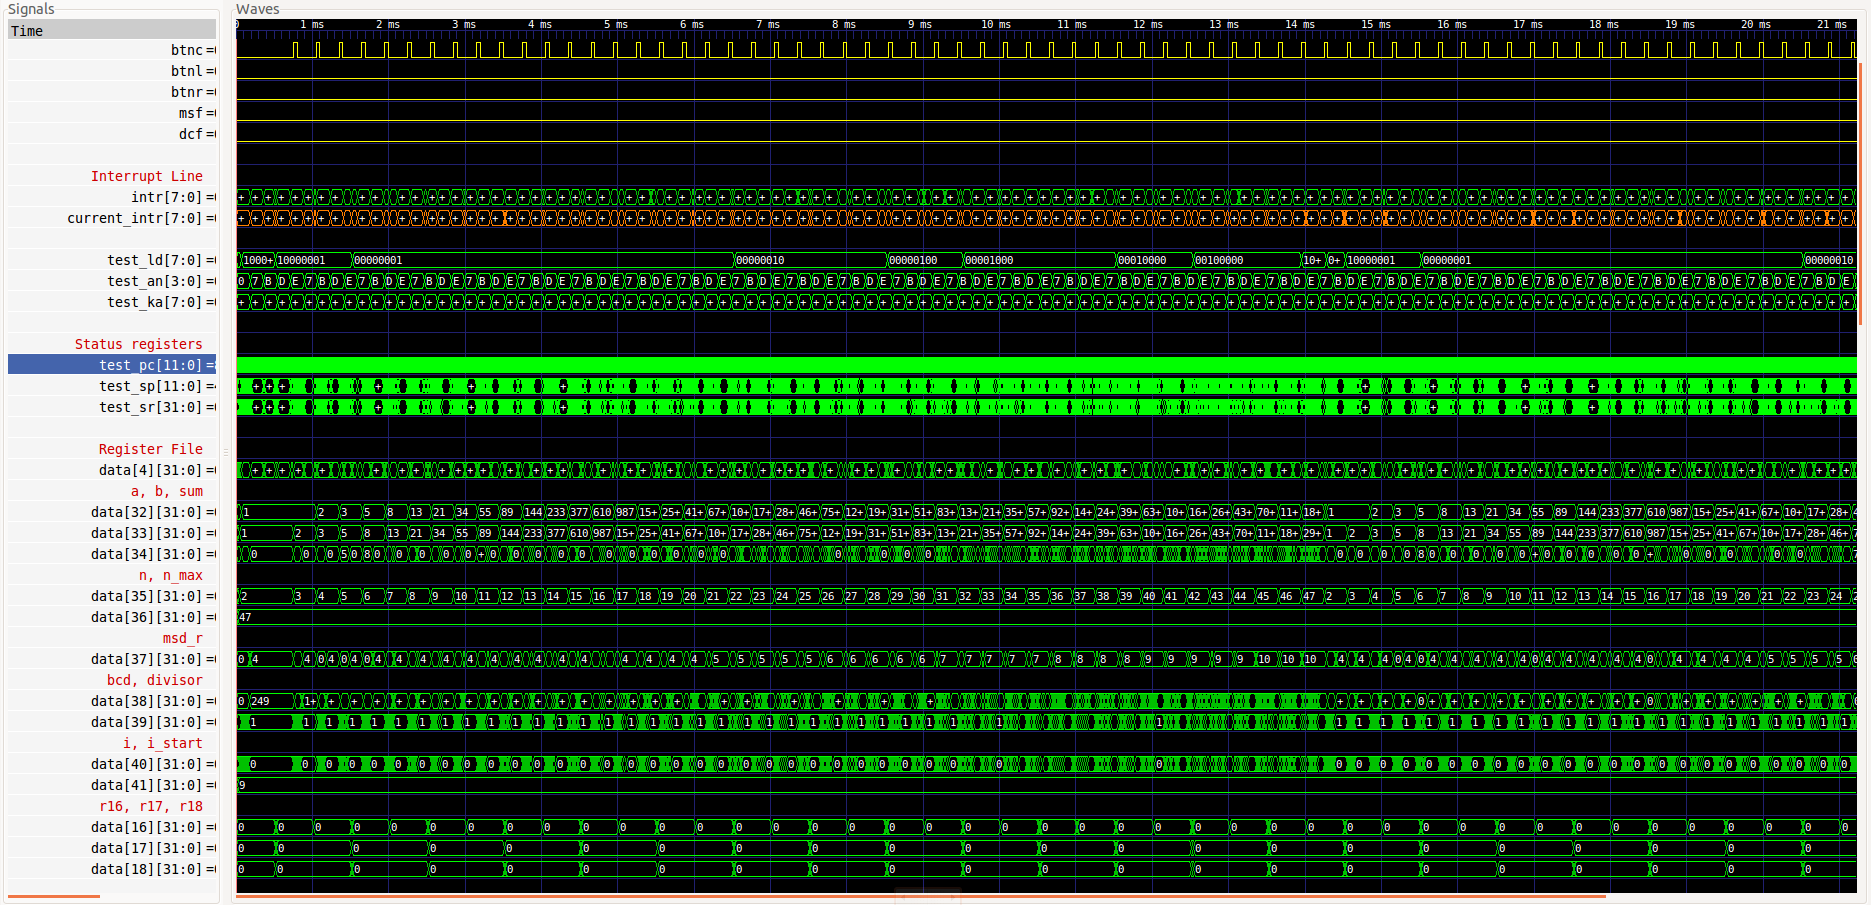
\includegraphics[width=7.2in]{assets/t0.png}
  \caption{All register and memory values over a course of 25 ms of
    sustained input.}
\end{figure}

\begin{figure}[H]
  \centering
  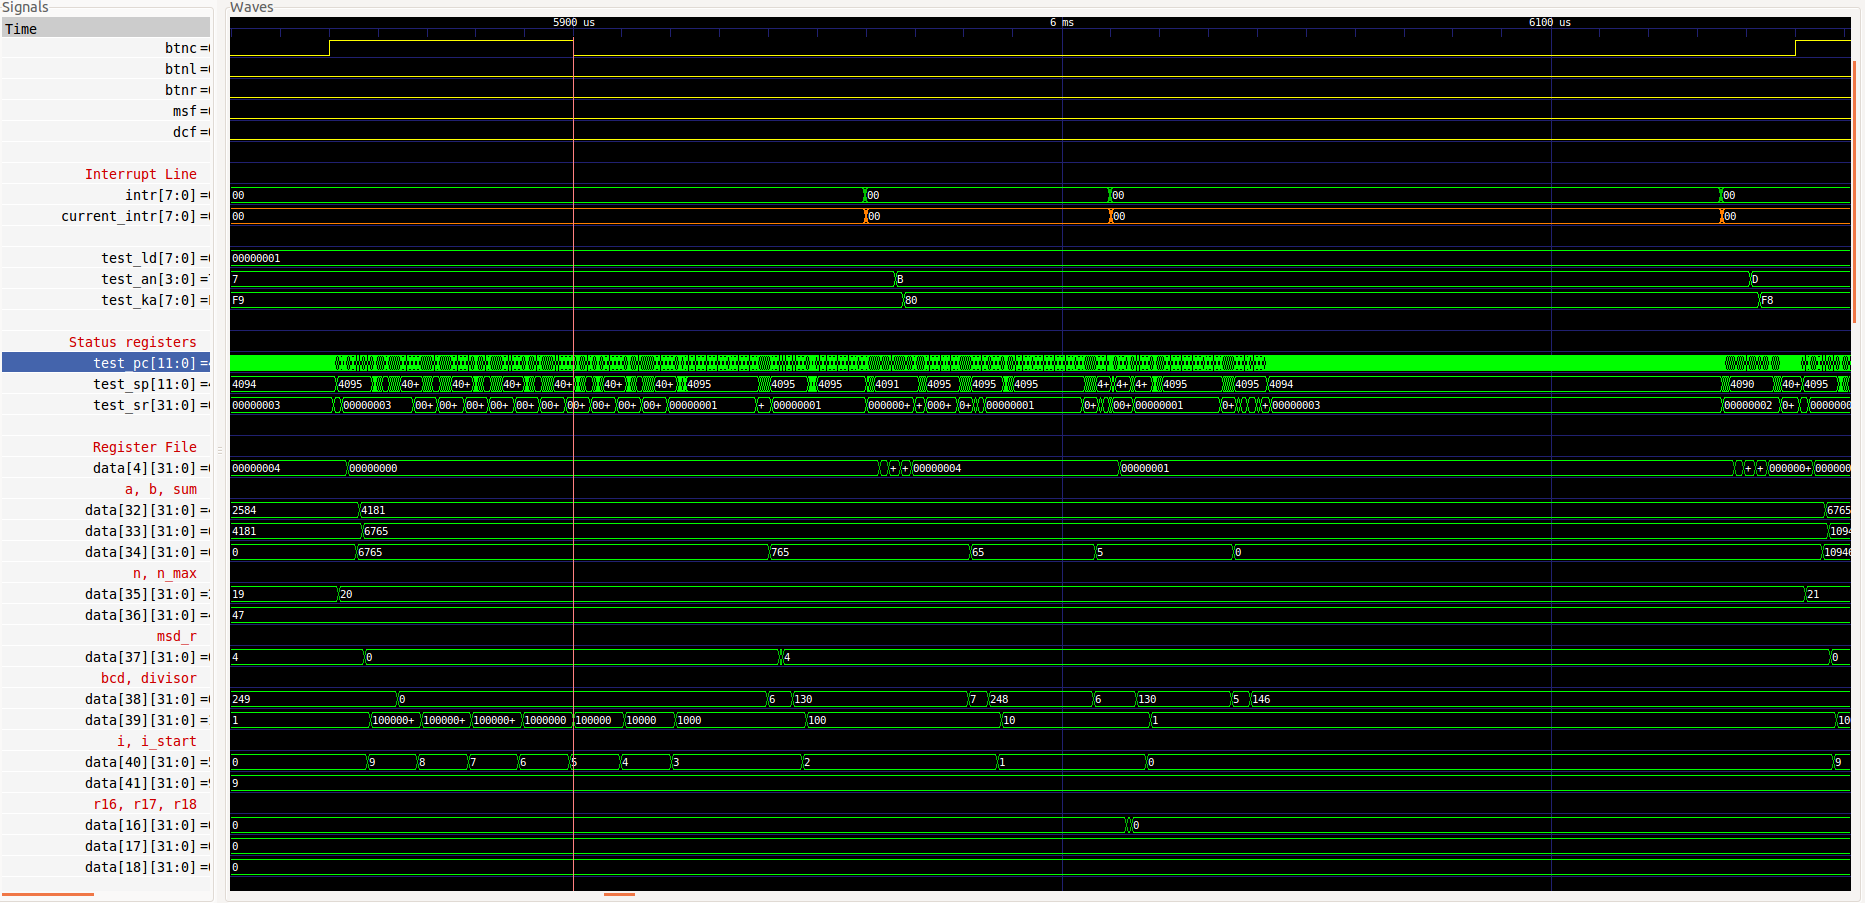
\includegraphics[width=7.2in]{assets/t1.png}
  \caption{Correct calculation of the next Fibonacci series number on
    centre button press.}
\end{figure}

\begin{figure}[H]
  \centering
  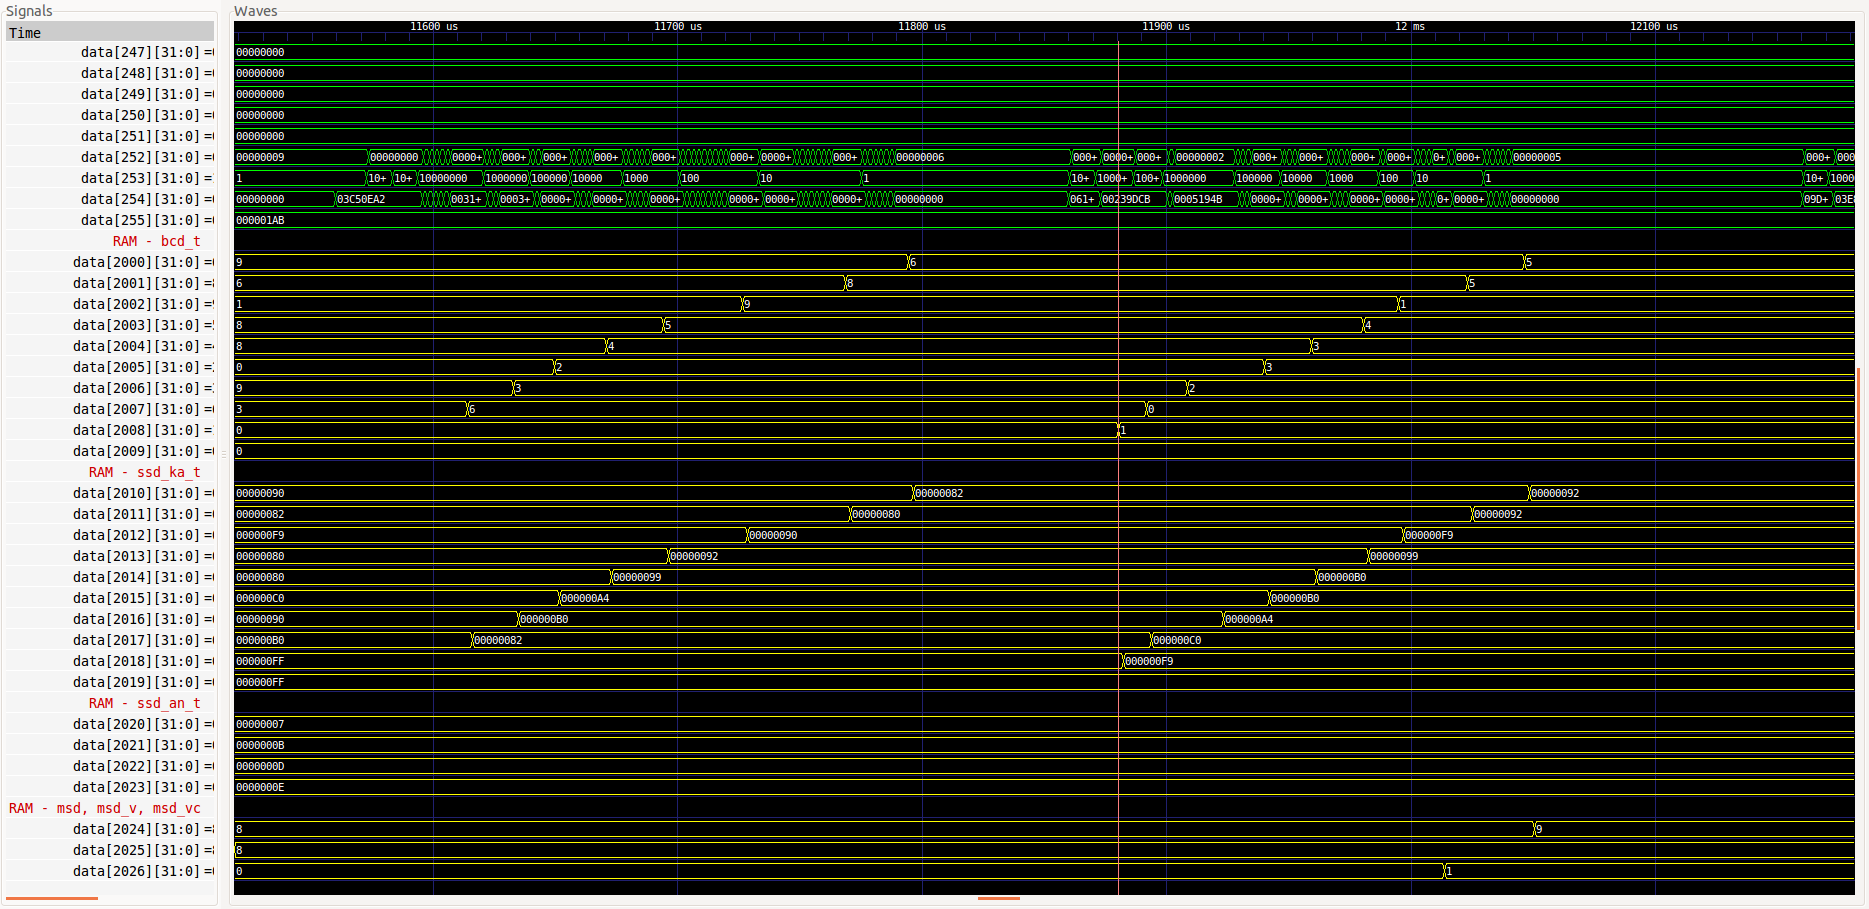
\includegraphics[width=7.2in]{assets/t2.png}
  \caption{Iterative binary to BCD conversion and translation into SSD
    cathode masks.}
\end{figure}

\begin{figure}[H]
  \centering
  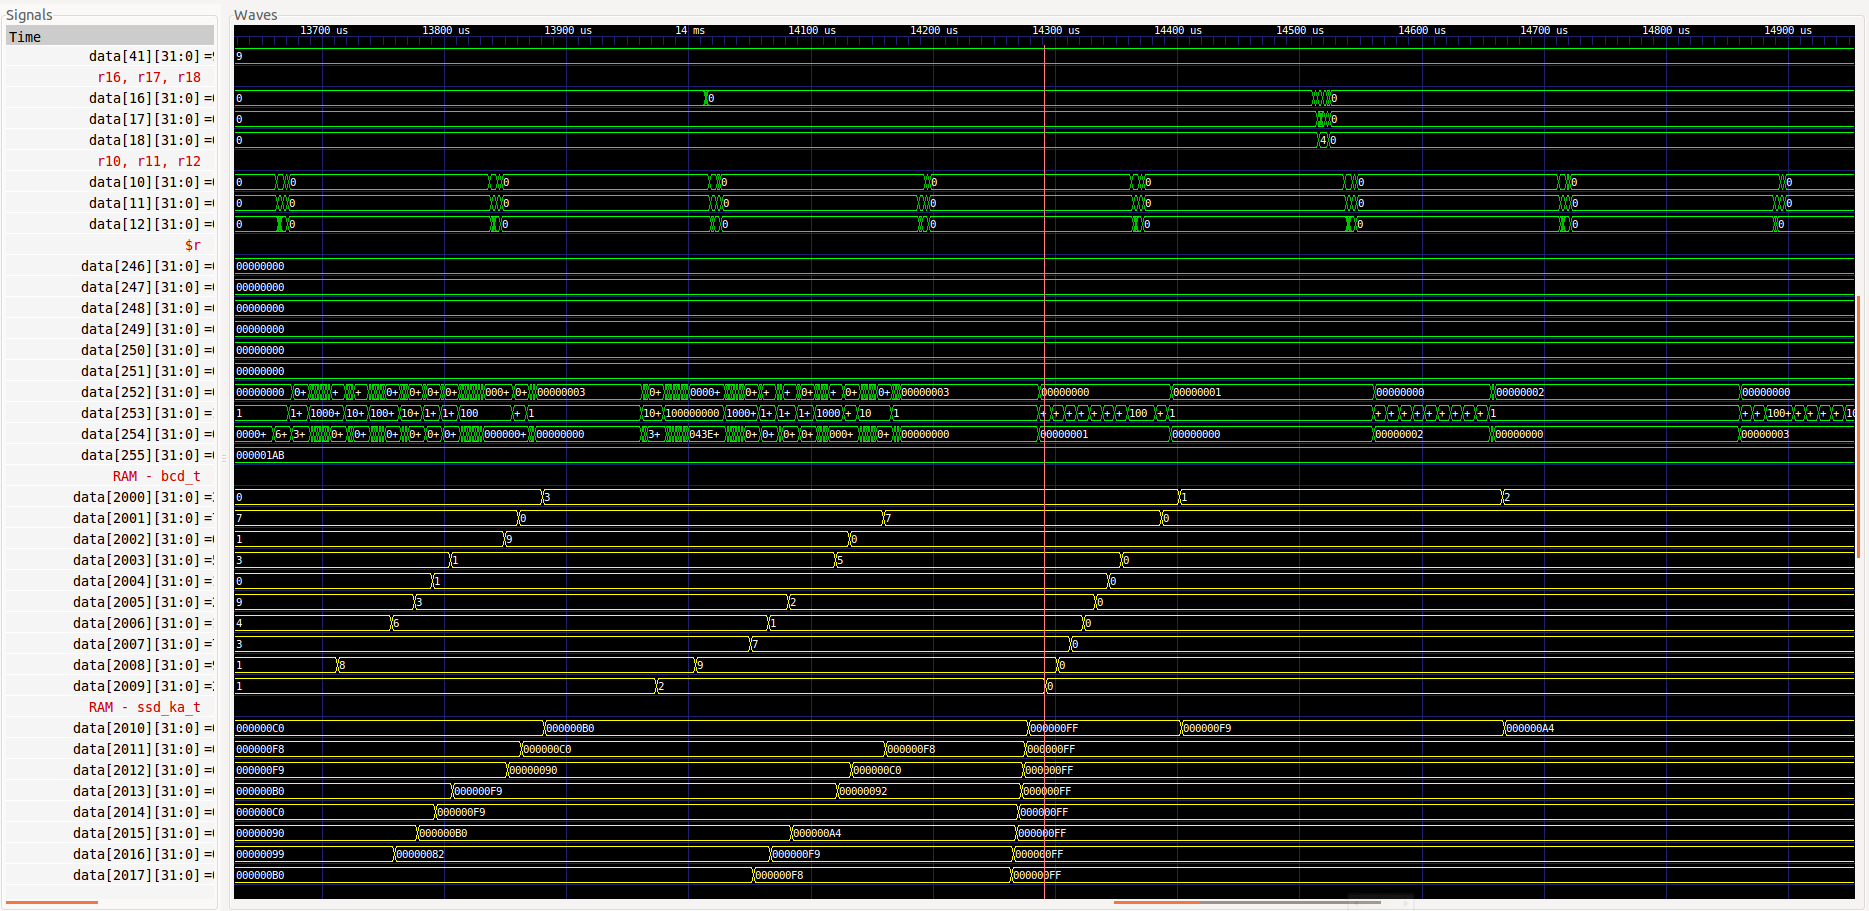
\includegraphics[width=7.2in]{assets/t3.png}
  \caption{Correct series reset every 47 button presses.}
\end{figure}

\begin{figure}[H]
  \centering
  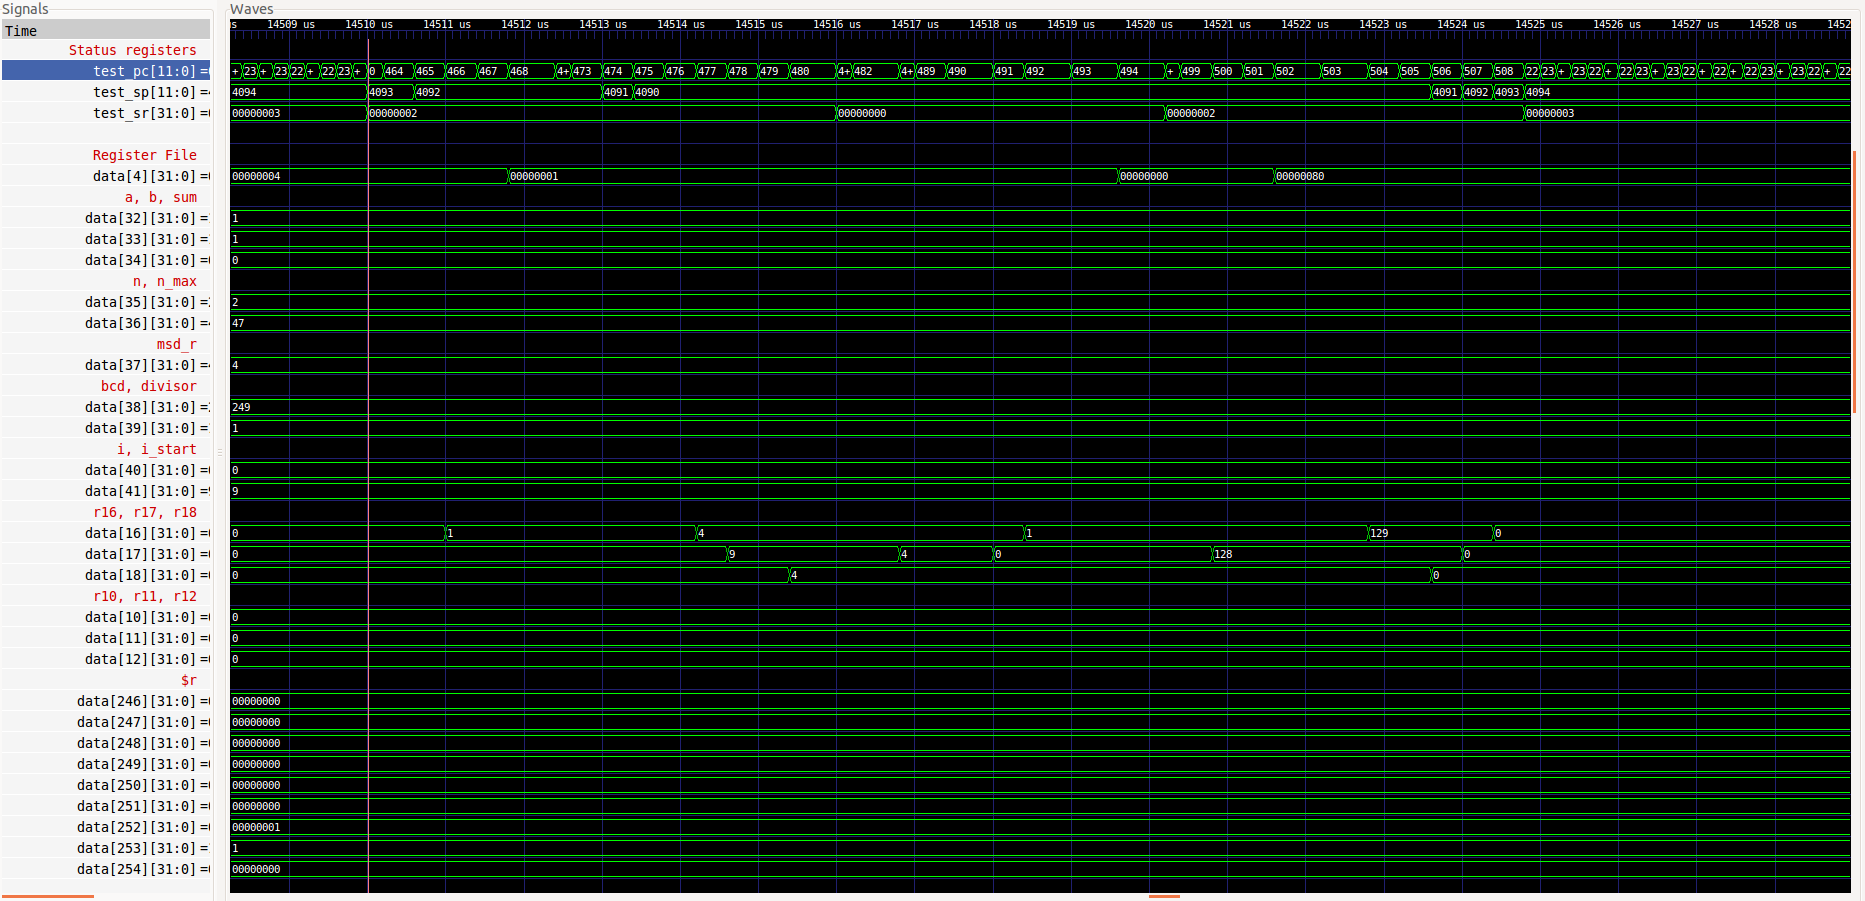
\includegraphics[width=7.2in]{assets/t4.png}
  \caption{Interrupt 0 handler correctly updating the currently
    visible SSD digits.}
\end{figure}

\begin{figure}[H]
  \centering
  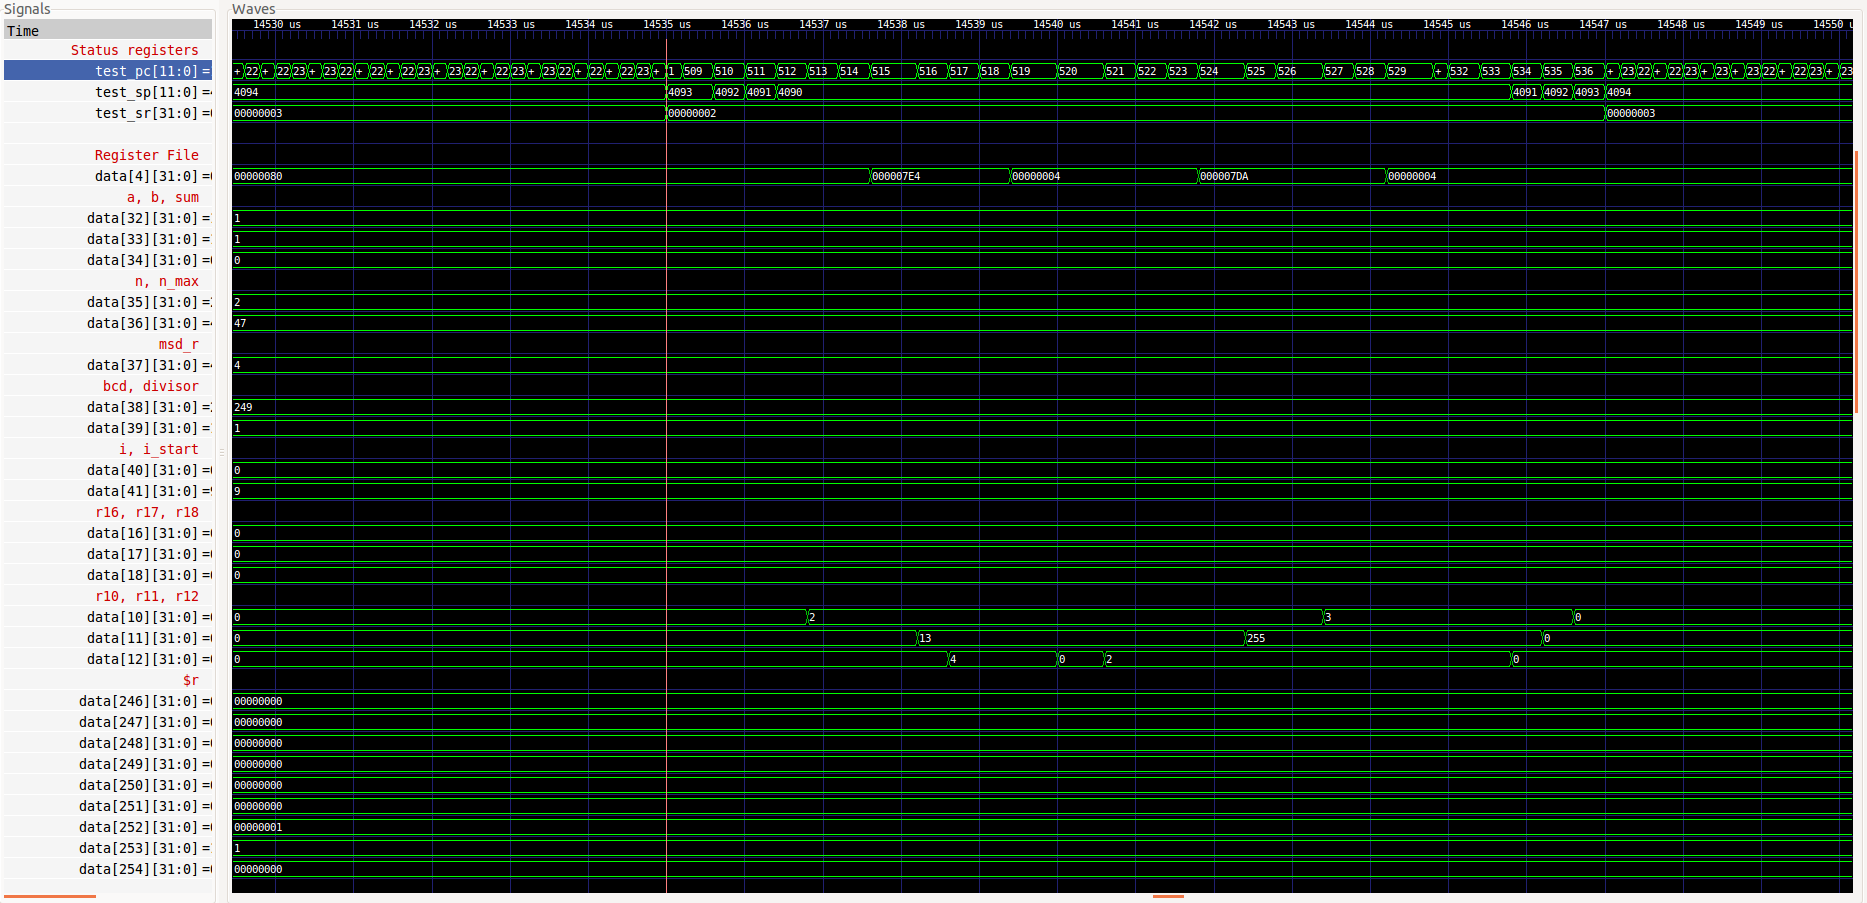
\includegraphics[width=7.2in]{assets/t5.png}
  \caption{Interrupt 1 handler setting the SSD anode and cathode
    ports.}
\end{figure}

The testbench is invoked from a modified Makefile which first
assembles the RAM file. Unlike previous testbenches, the signals are
not tested against expected outputs, but instead simple visual
confirmation of the correct values on the output ports can be used to
verify correct program functionality. The reason for this is that the
value of internal registers and signals are of little interest except
when debugging the assembler toolchain or detecting bugs in the
application code.

\begin{verbatim}
$ time make asm sim
./assembler/ucasm.js -s ram.asm -o ram.dat --annotate
ram.asm: 581 words, 14.185% util (cseg: 92% dseg: 8%)
...
ghdl -r test_bench --wave=test_bench.ghw
make asm sim  725.57s user 2.70s system 99% cpu 12:15.17 total
\end{verbatim}

\section{Hardware testing}

\end{document}
